\chapter{Simulation der Systemeigenschaften}
\label{chap4}
Ziel dieser Arbeit soll der Vergleich verschiedener Kombinationen von Ladesystem und Speichertechnologie aus technischer Sicht ein. Qualitative Bewertungen einer Kombination sind teilweise ohne Rechnung möglich (z. B. "`\textsc{Primove} ist besser für Lithium-Titanat-Batterien geeignet als für Lithium-Eisenphosphat-Batterien"'). Eine genauere Betrachtung und ein Vergleich von ähnlichen Technologiekombinationen ist jedoch nicht möglich. Daher werden in dieser Arbeit mit Hilfe eines Simulationsmodell quantitative Daten zu den verschiedenen Technologiekombinationen ermittelt.

\section{Simulationsmodell}
\marginpar{Ausfüllen! Quelle?} Ausgangspunkt ist das existierende Elektrobus-Simulationsmodell des Fachgebiets MPM der TU Berlin. Es wurde im Rahneb einer xxx erstellt und 2010 um ein Klimamodell sowie xxx von yyy um ein Batteriemodell erweitert.

\subsection{Energieverbrauch}

\begin{figure}\centering
	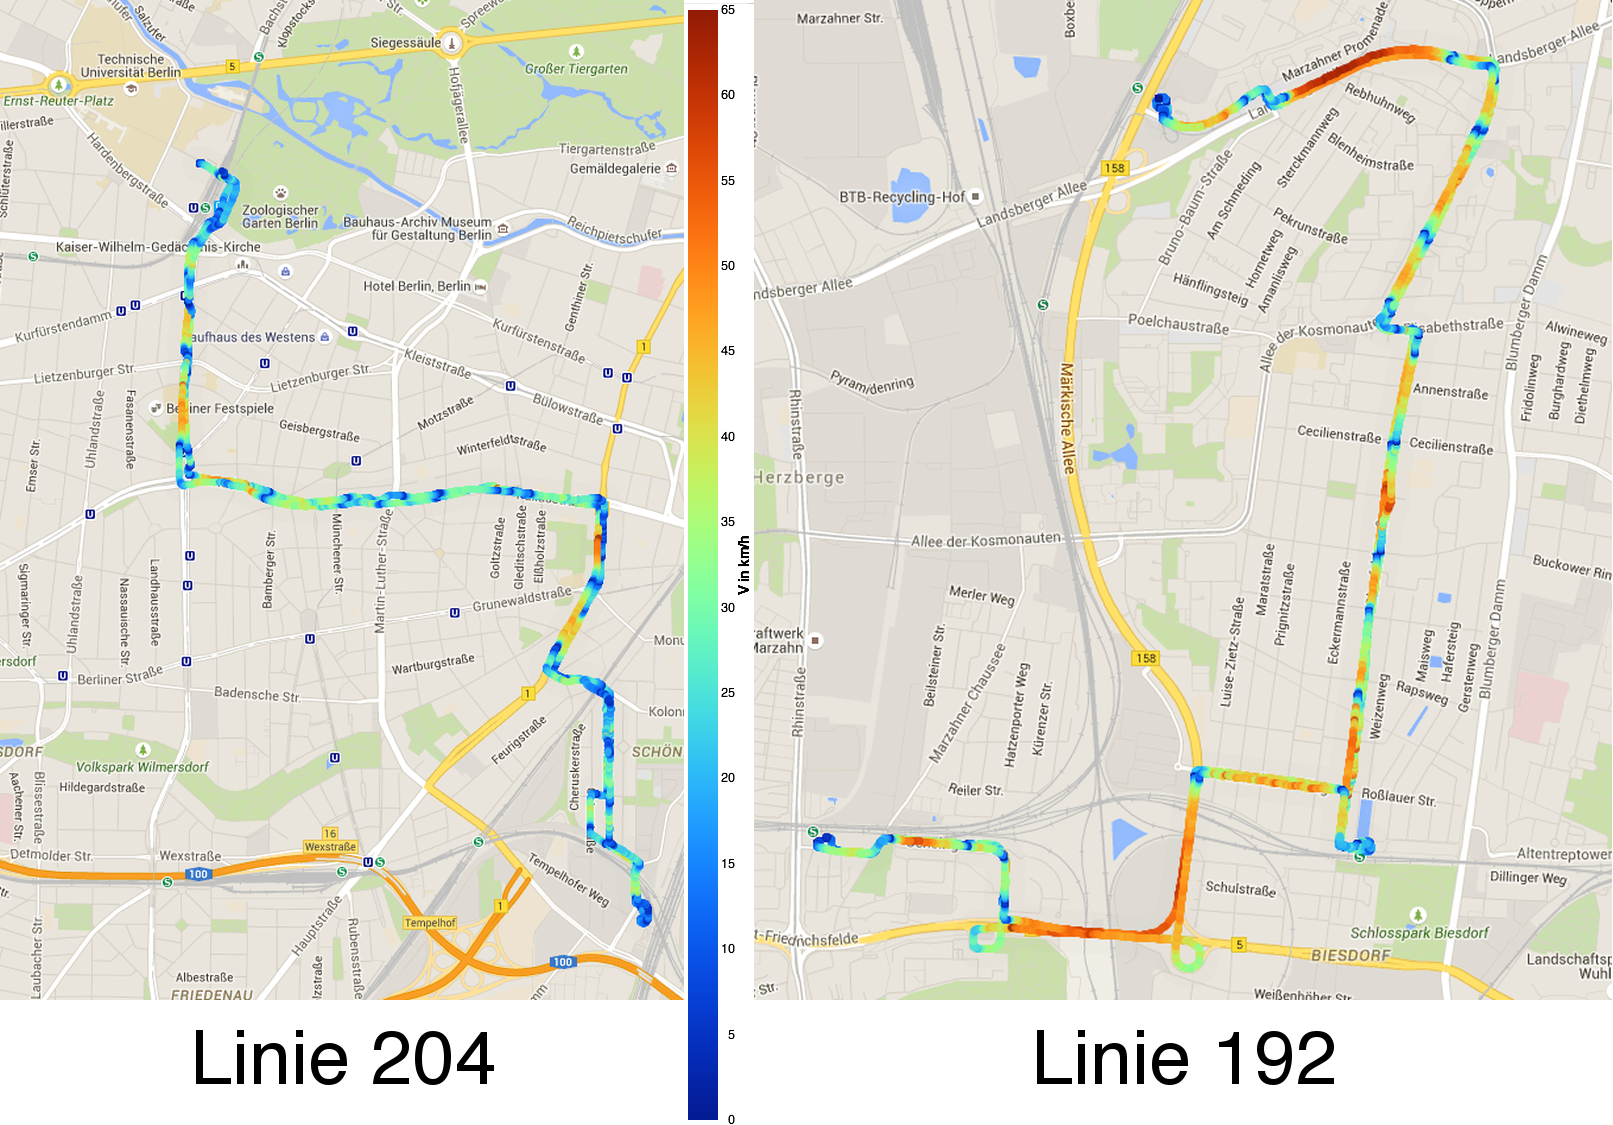
\includegraphics[width=\textwidth]{Buslinien}
	\caption[Verlauf und Geschwindigkeitsprofil der Buslinien]{Verlauf und Geschwindigkeitsprofil der Buslinien. Quelle: MPM TU Berlin}
	\label{Buslinien}
\end{figure}

Der erste Schritt der Simulation berechnet den Energieverbrauch aus einer aufgezeichneten Busfahrt. Die beiden verwendeten Aufzeichnungen sind in Abbildung \ref{Buslinien} zu sehen. In dieser Arbeit werden die Buslinien 204 und 192 der BVG betrachtet. die Buslinie 204 führt vom Bahnhof Zoo zum Südkreuz, sie ist eine innerstädtische Linie mit niedriger Durchschnittsgeschwindigkeit und vielen Beschleunigungs- und Bremsvorgängen. Die Linie 192 führt vom S-Bahnhof Marzahn zum S-Bahnhof Friedrichsfelde. Sie führt durch den Stadtrand, wie in der Abbildung ersichtlich ist hier die Durchschnittsgeschwindigkeit höher und das Geschwindigkeitsprofil gleichmäßiger.

Dabei werden die Geschwindigkeit, Höhe und Passagierzahl als Variablen sowie die Parameter des Busses als Konstanten verwendet. Mit den mechanischen Gesetzen zu Beschleunigung und Widerständen wird die zu jedem Zeitpunkt erforderliche Antriebsleistung mit einer Auflösung von einer Sekunde ermittelt. Über eine von xxx \marginpar{Quelle!} audgelegtes Motormodell wird aus der Wellenleistung die erforderliche elektrische Leistung und die verfügbare Rekuperationsleistung beim Bremsen berechnet.

\subsubsection{Nebenverbraucher}
Neben Antrieb entfällt ein signifikanter Teil der Batterieleistung auf die sogenannten Nebenverbraucher. Der weitaus wichtigste Nebenverbraucher ist die Klimatisierung des Busses. Die Kühlung erfolgt wie in einem Dieselbus durch eine elektrische Klimaanlage\marginpar{korrekt?} mit einer maximalen Leistung von xx kW. Für die Heizung kann jedoch nicht die Abwärme des Motors benutzt werden, da der Elektromotor dafür viel zu effizient ist. Von daher wird der Bus direkt geheizt, was im Winter eine Heizleistung von durchschnittlich 10 kW erfordert. Da die Heizleistung im Winter über der Kühhleistung im Sommer leigt, wird für diese Simulation die Heizleistung verwendet.

Für die anderen Nebenverbraucher wie Licht, Türen und Druckluft werden mit einer durchschnittlichen Leistung von 2 kW veranschlagt.

\subsection{Batteriemodell}
Da der Stromverbrauch durch, Strecke und Nebenverbraucher festgelegt ist, \emph{muss} die Batterie die geforderte Fahrleistung liefern. Sie \emph{kann} bis zu ihrer maximalen Ladeleistung Rekuperationsenergie nutzen. Darüber hinaus anfallende Bremsenergie wird in der Realität über einen Bremswiderstand auf dem Dach abgeleitet, in der Simulation wird sie ignoriert.

Im Modell existierte nur eine Modell für Lithium-Einsenphosphat-Batterien. Es entspricht dem empirischen Model von Lam und Bauer \cite{lam2011practical}. Dieses Modell stellt eine Lithium-Eisenphosphat-batterie in hoher Qualität dar, ist jedoch für andere Batterietypen ungeeignet.

Daher in dieser Arbeit das empirische Modell von Tremblay und Dessaint verwendet \cite{tremblay2009experimental}. Dieses Modell liefert weniger exakte Daten, kann aber dafür verschiedene Batterietypen darstellen. Ein großer Vorteil dieses Modells ist, das sich die Parameter der aus den Datenböättern der Batterien ablesen lassen. Damit kann man das Modell verschiedenen Batterietypen anpassen, ohne die Batterien selbst zu vermessen.

\subsubsection{Dimensionierung}
Die simulierte Batterie ist aus mehreren Zellen zusammengesetzt\footnote{Diese Zellen entsprechen nicht unbedingt einer chemischen Batteriezelle, sondern der kleinsten Batterie, die einzeln verfügbar ist.}. Durch iterative Optimierung wird die niedrigstmögliche Zellenzahl festgestellt. Als Randbedingung für die Optimierung wird ein maximaler und minimaler Ladezustand der Batterie verwendet. Daneben darf der maximale Entladestrom laut Datenblatt nicht überschritten werden.

\subsubsection{Ladesystem}
Im ursprünglichen Modell war die Ladezeit durch die aufgezeichnete Strecke festgelegt und nicht variabel. Da in dieser Arbeit die Ladezeiten verschiedener Technologiekombinationen verglichen werden sollen, wurde ein separates Modell für den Ladevorgang erstellt. Es besteht aus dem Batteriemodell und einer Energiequelle, die nach einer Totzeit die maximale Ladeleistung bereitstellt. Die Batterie nimmt entsprechend ihrer Ladekurve diese Leistung teilweise oder vollständig auf. Wenn die Batterie den gewünschten Ladezustand erreicht hat, endet die Simulation und die Ergebnisse können entnommen werden.

\subsection{Wärmeberechnung}
Der Abtransport der an der Batterie entstehenden Wärme stellt eine große Herausforderung bei der Auslegung eines Speichersystems dar. Durch Überhitzung kann die Batterie zerstört werden. Aber auch zulässige, aber innerhalb des Batteriepacks unterschiedliche Temperaturen führen zu einer unterschiedlichen Lebensdauer der verschiedenen Zellen und reduzieren so die Gesamtlebensdauer. Von daher wird in dieser Simulation auch die Größe des erforderlichen Kühlsystems abgeschätzt.

Wie in Abschnitt \ref{sec_waermeverluste} erläutert überwiegt bei hohen Strömen die vom Innenwiderstand verursachte irreversible Erwärmung. Bei niedrigen Strömen ist der Anteil der reversiblen Erwärmung höher, die Gesamterwärmung jedoch niedriger. Daher wird zur Abschätzung nur der irreversible Anteil mit einem Sicherheitsfaktor von 2 verwendet. Die Erwärmung der Batterien wird mit der Batteriemasse aus dem entsprechenden Datenblatt und den von Pesaran ermittelten Wärmekapazizäten berechnet~\cite{pesaran2001battery}.

Es wird eine parallele Luftkühlung verwendet, bei der die jeweils Luft nur an einer Zelle vorbeigeführt wird. Diese Methode wird von Pesaran als einfache Möglichkeit für eine gleichmäßige Temperatur im Batteriepack empfohlen~\cite{pesaran2001battery}. Es wird angenommen, das die Hälfte der Temperaturdifferenz zwischen Batterie und Umgebungsluft zur Kühlung verwendet werden kann. Als Umgebungstemperatur wird ein Wert von 40 $^{\circ}C$ angenommen, der noch eine kleine Reserve zur höchsten in Berlin gemessenen Temperatur von 38,1 $^{\circ}C$ bietet\cite{tempRekord}. Die benötigte Luftmenge wird mit durch einem PD-Regler berechnet und der Höchstwert in $\frac{g}{s}$ angegeben.

Es wird nicht unbedingt die ideale Kühlung für jede mögliche Batterie verwendet, sondern es werden vergleichbare Werte für verschiedene Batterien berechnet, in denen Masse, Wärmekapazität und Maximaltemperatur zusammengefasst sind.

\section{Ergebnisse}

Aus den unzähligen Ausgabedaten der Simulation wurden die folgenden ausgewählt, um die Kombinationen von Lade- und Speichersystem zu vergleichen:
\begin{description}
	\item[Batteriemasse] Einheit: $kg$
	\item[Batterivolumen] Einheit: $l$
	\item[Kühlluftmasse] Dieser Wert sollte nicht zur Auslegung eines Kühlsystems verwendet werden, sondern nur zum Vergleich der Lösungen untereinander.\\
	Einheit: $\frac{g}{s}$
	\item[Energieverbrauch] Einheit: $\frac{kWh}{km}$
	\item[Zeiteffizienz] Der Anteil der Ladezeit an der Summe von Fahr- und Ladezeit. Kleinere Werte sind besser.
	Einheit: $1$ bei Gelegeheitsladung, $h$ bei Nachtladung
	\item[Ladezyklen pro Kilometer] Mit diesem Wert kann der Einfluss dieser Kobination auf die Lebensdauer der Batterie abgeschätzt werden.
	Einheit: $1$
\end{description}

\subsection{Linie 204}
\subsubsection{Nachtladung}
Bei der Ladestrategie "`Nachtladung"' fährt der Bus tagsüber ohne Zwischenladen auf der Strecke. Er absolviert 11 Touren mit einer Gesamtlänge von 132 $km$. Die Batterie darf sich dabei auf maximal 10\% Ladezustand entladen. Nach Betriebsschluss wird der Bus über Nacht im Depot auf 100\% Ladezustand geladen. Als Ladesystem wurde ein konduktiv-manuelles System mit 40kW gewählt.

\begin{table}[h!]\centering
	\begin{tabularx}{\textwidth}{Xrrrrrr}
		\toprule
		Batterie    & Masse & Volumen &       Kühlung &          Energie & Ladezeit & Ladezyklen \\
		            &  $kg$ &     $l$ & $\frac{g}{s}$ & $\frac{kWh}{km}$ &      $h$ &        $1$ \\ \midrule
		18650 &  681 &     246 &           1673 &              1,20 &       4,7   & 0,0063 \\
		Bleiakku    & 8217 &    3082 &           512 &              1,91 &      9,5    & 0,0063 \\
		LiTiO       &  2174 &    1522 &             190 &              1,26 &       4,9   & 0,0062 \\
		LiFePO-HE      &  1214 &    736 &          5254 &              1,16 &       4,0   & 0,0063 \\ 
		LiFePO-HP      &  1577 &    824 &          4941 &              1,24 &       5,0  & 0,0063 \\ \bottomrule
	\end{tabularx}
	\caption{Simulationsergebnisse Nachtladung}
\end{table}
\FloatBarrier
\subsubsection{Gelegenheitsladung}
Bei der Ladestrategie "`Gelegenheitsladung"' wird der Bus nach jeder Folge von Hin- und Rückfahrt aufgeladen. Die Länge einer Tour beträgt 12 $km$. Bei dieser Ladestrategie werden sämtliche Ladesysteme betrachet.

\begin{table}[h!]
	\begin{minipage}{0.45\textwidth}
		\centering
		\begin{tabular}{lrrrrr}
			\multicolumn{5}{c}{Batteriemassen in $kg$} \\ \toprule
			Bat./LS     & 40kW & 200kW &         375kW & Swap\\ \midrule
			18650 &  247 &   257 &           249 & \\
			Bleiakku    & 1944 &  1944 &          1944 & \\
			LiTiO       &  693 &   695 &           694 & \\
			LiFePO      &  434 &   434 &           434 & \\ \bottomrule 
		\end{tabular} 
		\caption{Batteriemassen Gelegnheitsladung}
		
		\begin{tabular}{lrrrrr}
			 & & & & \\
			\multicolumn{5}{c}{Kühlbedarf in $\frac{g}{s}$} \\ \toprule
			Bat./LS     & 40kW & 200kW &              375kW & Swap\\ \midrule
			18650 &  206 &   197 &                207 & \\
			Bleiakku    & 1342 &  1381 &               1351 & \\
			LiTiO       &  504 &  1220 &               1217 & \\
			LiFePO      & 5096 &  5154 &               5110 & \\ \bottomrule 
		\end{tabular} 
		\caption{Kühlungsbedarf Gelegenheitsladung}
		
		\begin{tabular}{lrrrr}
			 & & & & \\
			\multicolumn{5}{c}{Anteil Ladezeit an Gesamtzeit} \\ \toprule
			Bat./LS     & 40kW & 200kW &                375kW & Swap\\ \midrule
			18650 & 0,38 &  0,37 &                 0,38 & \\
			Bleiakku    & 0,64 &  0,64 &                 0,64 & \\
			LiTiO       & 0,33 &  0,12 &                 0,12 & \\
			LiFePO      & 0,33 &  0,23 &                 0,23 & \\ \bottomrule 
		\end{tabular} 
		\caption{Ladezeitanteil Gelegenheitsladung}
		
	\end{minipage}\hfill
	\begin{minipage}{0.45\textwidth}
		\centering
		\begin{tabular}{lrrrr}
			\multicolumn{5}{c}{Batterievolumina in $l$} \\ \toprule
			Bat./LS     & 40kW & 200kW &          375kW & Swap\\ \midrule
			18650 &   90 &    93 &             90 & \\
			Bleiakku    &  729 &   729 &            729 & \\
			LiTiO       &  485 &   487 &            486 & \\
			LiFePO      &  263 &   263 &            263 & \\ \bottomrule 
		\end{tabular}
		\caption{Batterievolumina Gelegenheitsladung}
		
		\begin{tabular}{lrrrr}
			 & & & & \\
			\multicolumn{5}{c}{Energieverbrauch in $\frac{kWh}{km}$} \\ \toprule
			Bat./LS     & 40kW & 200kW &                       375kW & Swap\\ \midrule
			18650 & 2.16 &  2.23 &                        2.16 & \\
			Bleiakku    & 2.66 &  2.77 &                        2.67 & \\
			LiTiO       & 1.98 &  2.21 &                        2.14 & \\
			LiFePO      & 2.02 &  2.12 &                        2.05 & \\ \bottomrule 
		\end{tabular} 
		\caption{Energieverbrauch Gelegenheitsladung}
		
		\begin{tabular}{lrrrr}
			 & & & & \\
			\multicolumn{5}{c}{Ladezyklen pro Kilometer} \\ \toprule
			Bat./LS     &  40kW & 200kW &          375kW & Swap\\ \midrule
			18650 & 0.030 & 0.029 &          0.030 & \\
			Bleiakku    & 0.036 & 0.037 &          0.037 & \\
			LiTiO       & 0.030 & 0.030 &          0.030 & \\
			LiFePO      & 0.030 & 0.030 &          0.030 & \\ \bottomrule 
		\end{tabular} 
		\caption{Ladezyklen pro Kilometer Gelegenheitsladung}	
		
	\end{minipage}
	
	
\end{table}

%\subsection{Linie M19}
%Lipsumsdkjfgasdjkhf \marginpar{TODO!}